\documentclass[11pt,letterpaper]{article}

\usepackage[margin=1in]{geometry}
\usepackage{setspace}
\onehalfspacing

\usepackage{microtype}
\usepackage{titlesec}
\usepackage{enumitem}
\usepackage{booktabs}
\usepackage{longtable}
\usepackage{multirow}
\usepackage{array}
\usepackage{tabularx}
\usepackage{xcolor}
\usepackage{colortbl}

\usepackage{tikz}
\usetikzlibrary{shapes.geometric, arrows.meta, positioning, fit, backgrounds, calc, decorations.pathreplacing, patterns, shadows}
\usepackage{pgfplots}
\pgfplotsset{compat=1.18}

\usepackage{amsmath,amssymb,amsthm}

\usepackage[colorlinks=true,linkcolor=blue,citecolor=blue,urlcolor=blue]{hyperref}
\usepackage{cleveref}

\usepackage[numbers,sort&compress]{natbib}

\definecolor{ucxblue}{RGB}{0,102,204}
\definecolor{ncclgreen}{RGB}{118,185,0}
\definecolor{cudaorange}{RGB}{255,153,0}
\definecolor{rdmared}{RGB}{204,0,0}
\definecolor{solutiongreen}{RGB}{40,167,69}
\definecolor{layergray}{RGB}{240,240,240}
\definecolor{dbpurple}{RGB}{102,51,153}
\definecolor{v100blue}{RGB}{30,90,180}
\definecolor{tower1color}{RGB}{50,130,60}
\definecolor{tower2color}{RGB}{130,50,50}

\theoremstyle{definition}
\newtheorem{challenge}{Challenge}
\newtheorem{designchoice}{Design Choice}

\title{
    \vspace{-1cm}
    \textbf{Adaptive RDMA Optimization for Distributed LLM Workloads} \\[0.5em]
    \large Update 8: RDMA Tensor Cache Architecture and Database Design
}

\author{
    Nathan Gopee \\
    \textit{MS Computer Science Candidate} \\
    SUNY New Paltz \\
    \texttt{gopeen1@newpaltz.edu} \\[1em]
    \small Advisors: Dr.\ Wafi Danesh \& Dr.\ Ashley Suchy
}

\date{February 2026}

\begin{document}

\maketitle

\begin{abstract}
\noindent
Heterogeneous GPU clusters present a precision mismatch problem that fundamentally limits distributed LLM training and inference. This update presents the RDMA Tensor Cache, a centralized precision management layer implemented within the tensor database, designed for a two-tower home lab: Tower~1 (Ryzen~9~7950X, RTX~5070~Ti~16GB, Windows) and Tower~2 (Proxmox/Linux, $2\times$ Tesla~V100~32GB). The V100s lack BF16 support, forcing FP16 computation with its narrow dynamic range; the 5070~Ti supports BF16 natively but runs on Windows without kernel RDMA. We resolve this with an RDMA-accessible FP32 master weight store in the tensor database, stochastic rounding for precision-lossy conversions, predictive tensor prefetching, and a centralized KV cache that eliminates the per-rank duplication problem inherent to Multi-Latent Attention (MLA) and Multi-Query Attention (MQA) under tensor parallelism. We detail the \texttt{tensor\_rdma} crate architecture, present three experimental pillars for validation, and describe integration paths through UCX/UCC, SoftRoCEv2, and the emerging Ultra Ethernet Consortium (UEC) 1.0 standard.
\end{abstract}

\tableofcontents
\newpage

%=============================================================================
\section{Overview}
\label{sec:overview}
%=============================================================================

This update advances the thesis in three directions. First, we formalize the RDMA Tensor Cache architecture that bridges the precision gap between V100 and 5070~Ti GPUs by centralizing master weights in the tensor database's \texttt{tensor\_rdma} crate. Second, we analyze the parallelism strategies available in vLLM and identify a structural limitation of tensor parallelism for MLA/MQA models that motivates our centralized KV cache design. Third, we introduce Sparse Auto-Encoders (SAEs) as an alternative to gradient-based fine-tuning, showing how SAE feature vectors map naturally to the tensor database's \texttt{SparseVector} representation with 51$\times$ compression.

The home lab consists of two towers connected by Mellanox ConnectX-4 100GbE NICs:

\begin{table}[htbp]
\centering
\caption{Home lab hardware configuration}
\label{tab:hardware}
\begin{tabular}{@{}lll@{}}
\toprule
\textbf{Component} & \textbf{Tower 1 (Windows)} & \textbf{Tower 2 (Proxmox/Linux)} \\
\midrule
CPU & Ryzen 9 7950X (16c/32t) & Xeon (host CPU) \\
RAM & 192 GB DDR5 & Host RAM \\
GPU & RTX 5070 Ti 16 GB (compute 12.0) & $2\times$ Tesla V100 32 GB \\
NIC & Mellanox ConnectX-4 100GbE & Mellanox ConnectX-4 100GbE \\
OS & Windows 11 & Proxmox (Debian/Linux) \\
RDMA & TCP/gRPC fallback (no kernel RDMA) & SoftRoCEv2 / GPUDirect RDMA \\
BF16 & Native & Not supported \\
FP16 & Supported & Native compute \\
IP & -- & 192.168.2.111 (South-Tower) \\
\bottomrule
\end{tabular}
\end{table}

The fundamental tension is that the V100 is a datacenter GPU with full GPUDirect RDMA support and Tensor Core FP16 compute but no BF16, while the 5070~Ti is a consumer GPU with BF16 native support but no RDMA stack on Windows. The RDMA Tensor Cache resolves this asymmetry by placing FP32 master weights in the tensor database, accessible from both towers through different transport paths.

%=============================================================================
\section{NVIDIA Open-Source Ecosystem}
\label{sec:nvidia-ecosystem}
%=============================================================================

The NVIDIA communication stack comprises several interdependent libraries that form the foundation for GPU-accelerated distributed computing. Understanding their boundaries and transport mechanisms is essential for positioning the RDMA Tensor Cache within the ecosystem.

\subsection{NCCL}

NCCL~\cite{nccl} provides collective communication primitives (AllReduce, AllGather, ReduceScatter, AllToAll) optimized for multi-GPU training. It operates at the collective level and handles topology detection, ring/tree algorithm selection, and NVLink/PCIe/InfiniBand transport. NCCL is tightly coupled to NVIDIA hardware---it uses CUDA kernels for data packing and relies on \texttt{cudaIpcGetMemHandle} for intra-node peer-to-peer transfers.

For our cluster, NCCL can drive the V100-to-V100 communication path on Tower~2. However, NCCL cannot bridge heterogeneous precision natively; it transmits tensors in their source format without conversion.

\subsection{UCX and HPC-X}

UCX (Unified Communication X)~\cite{ucx} is a point-to-point communication framework providing transport-agnostic abstractions over InfiniBand, RoCE, TCP, and shared memory. HPC-X v2.15~\cite{hpcx} bundles UCX with optimized MPI and collective layers. UCX exposes several transport modes relevant to our ConnectX-4 NICs:

\begin{table}[htbp]
\centering
\caption{UCX transport modes for ConnectX-4}
\label{tab:ucx-transports}
\begin{tabular}{@{}llp{7.5cm}@{}}
\toprule
\textbf{Transport} & \textbf{Mode} & \textbf{Description} \\
\midrule
RC & Reliable Connection & One QP per peer. Guaranteed delivery with retransmission. Default for multi-node. \\
DC & Dynamic Connection & ConnectX-4+. Single QP multiplexed across peers. Reduces QP state for large clusters. \\
UD & Unreliable Datagram & Connectionless. Useful for short control messages but no reliability guarantees. \\
TCP & Socket Fallback & Standard TCP/IP. Cross-platform, available on Windows. \\
SHM & Shared Memory & Intra-node via \texttt{/dev/shm}. Lowest latency for same-host processes. \\
CUDA & GPU Memory & Direct GPU buffer access via \texttt{cuMemcpy} or GDR. Requires \texttt{nvidia-peermem}. \\
\bottomrule
\end{tabular}
\end{table}

The distinction between datacenter and consumer GPUs is critical here. The V100, as a datacenter-class GPU, supports GPUDirect RDMA: the NIC can DMA directly into GPU memory without staging through host RAM. The 5070~Ti, as a consumer GPU on Windows, must use TCP or gRPC as its transport, with data copied through system memory.

\subsection{GPUDirect RDMA and nvidia-peermem}

GPUDirect RDMA~\cite{gpudirect-rdma-redhat} enables RDMA NICs to read/write GPU memory directly. It requires the \texttt{nvidia-peermem} kernel module, which registers GPU memory regions with the InfiniBand subsystem. On Tower~2 (Linux), GPUDirect RDMA is configured by loading the \texttt{nvidia-peermem} kernel module and verifying that the module registers GPU peer memory successfully through kernel messages. The RDMA device information is then confirmed via \texttt{ibv\_devinfo}, which reports the ConnectX-4 NIC (\texttt{mlx5\_0}) with InfiniBand transport, firmware version 12.28.2006, and a single physical port. This confirms that the NIC can perform direct memory access to V100 GPU memory regions.

\subsection{GDRCopy}

GDRCopy~\cite{gdrcopy} provides a low-latency mechanism for CPU-initiated copies to/from GPU memory, complementing GPUDirect RDMA (which is NIC-initiated). For small tensors (control messages, metadata, KV cache headers), GDRCopy avoids the overhead of launching a CUDA kernel for the copy.

\subsection{NIXL}

NIXL (NVIDIA Inference Xfer Library)~\cite{nixl} provides point-to-point tensor transfer primitives for disaggregated inference. Where NCCL focuses on collective operations for training, NIXL targets the prefill/decode KV cache transfer pattern in serving systems. Its \texttt{NixlConnector} interface in vLLM serves as a reference for our middleware integration (Section~\ref{sec:python-prototype}).

\subsection{Megatron-LM}

Megatron-LM~\cite{megatron2020} established the canonical model parallelism strategies (tensor parallelism, pipeline parallelism, data parallelism) that all subsequent distributed training frameworks reference. Its tensor parallelism implementation shards weight matrices column-wise or row-wise across GPUs, requiring AllReduce after each transformer layer. This communication pattern directly informs our prefetch engine design.

Megatron-LM's approach to mixed precision training is particularly relevant: it maintains FP32 master weights on the optimizer node while broadcasting FP16 copies to compute nodes. Our RDMA Tensor Cache generalizes this pattern by placing the FP32 master store in the tensor database (accessible via RDMA) rather than requiring it to reside in GPU memory on a designated node. This decoupling enables the heterogeneous V100/5070~Ti configuration where no single GPU type can serve as the universal master.

\subsection{InfiniBand RDMA Foundations}

The RDMA programming model~\cite{infiniband-rdma} provides three key abstractions that \texttt{tensor\_rdma}'s transport layer mirrors:

\begin{enumerate}
    \item \textbf{Memory Registration:} Before RDMA operations, memory regions must be registered with the NIC via \texttt{ibv\_reg\_mr}. This pins physical pages and provides the NIC with a translation table. Our \texttt{register\_buffer} method models this step. Registration is expensive ($\sim$10~$\mu$s) but amortized across thousands of RDMA operations on the same buffer.

    \item \textbf{Queue Pairs (QPs):} Communication endpoints consisting of a Send Queue and Receive Queue. Our \texttt{TransportConfig::SoftRoce} configures QP parameters (device, GID index, port). The choice between Reliable Connection (RC) and Dynamic Connection (DC) QPs affects scalability: RC requires $O(n^2)$ QPs for an $n$-node cluster, while DC multiplexes a single QP across all peers.

    \item \textbf{One-Sided Operations:} RDMA Read and Write execute without involving the remote CPU. The initiating NIC issues the DMA directly to/from the remote NIC, which accesses the pre-registered memory region. This is why GPUDirect RDMA is so effective: the NIC writes directly into GPU BAR1 memory, bypassing both CPUs entirely. Our \texttt{rdma\_write} and \texttt{rdma\_read} methods map to \texttt{ibv\_post\_send} with \texttt{IBV\_WR\_RDMA\_WRITE} and \texttt{IBV\_WR\_RDMA\_READ} opcodes respectively.
\end{enumerate}

For a tensor of size $S$ bytes, the total transfer time over RDMA is:
\begin{equation}
    T_{\text{RDMA}} = T_{\text{latency}} + \frac{S}{B_{\text{link}}} + T_{\text{DMA}}
\end{equation}
where $T_{\text{latency}}$ is the one-way latency ($\sim$2~$\mu$s for hardware RoCE), $B_{\text{link}}$ is the link bandwidth (12.5~GB/s for 100GbE), and $T_{\text{DMA}}$ is the DMA engine overhead ($\sim$0.5~$\mu$s). For a 256~MB gradient tensor (typical for a transformer layer with hidden dimension 4096), $T_{\text{RDMA}} \approx 2 + 20480 + 0.5 \approx 20.5$~ms. This is dominated by bandwidth, not latency, confirming that 100GbE is the bottleneck rather than RDMA protocol overhead.

%=============================================================================
\section{vLLM Parallelism Analysis}
\label{sec:vllm-parallelism}
%=============================================================================

The choice between tensor parallelism (TP) and pipeline parallelism (PP) has significant implications for RDMA communication patterns and KV cache management. We analyze the trade-offs based on vLLM's architecture and community discussions~\cite{vllm-tp-pp-discussion}.

\subsection{Tensor Parallelism}

Tensor parallelism partitions weight matrices across GPUs within a single node. Each GPU computes a shard of the attention and MLP layers, then synchronizes via AllReduce. The communication volume per layer is:
\begin{equation}
    V_{\text{TP}} = 2 \cdot b \cdot s \cdot h \cdot (\text{TP} - 1) / \text{TP}
\end{equation}
where $b$ is batch size, $s$ is sequence length, $h$ is hidden dimension, and TP is the tensor parallel degree. This AllReduce occurs \emph{within} each transformer layer, making it latency-sensitive: any delay propagates through all layers.

For Tower~2 with $2\times$ V100, TP=2 is natural. The two GPUs communicate via PCIe (no NVLink on our configuration), so AllReduce latency is dominated by PCIe bandwidth ($\sim$12 GB/s bidirectional per GPU).

\subsection{Pipeline Parallelism}

Pipeline parallelism assigns contiguous blocks of transformer layers to different GPUs. Communication occurs only at pipeline stage boundaries, transmitting activations forward and gradients backward. The communication volume per micro-batch is:
\begin{equation}
    V_{\text{PP}} = b \cdot s \cdot h
\end{equation}
which is independent of the parallelism degree. However, pipeline parallelism introduces the \emph{pipeline bubble}---time during which GPUs are idle waiting for upstream stages to complete. The bubble fraction for a $p$-stage pipeline with $m$ micro-batches is:
\begin{equation}
    \text{Bubble} = \frac{p - 1}{m + p - 1}
\end{equation}

For cross-node communication (Tower~1 to Tower~2), PP is preferable because it moves communication out of the critical per-layer path. The 100GbE link has higher latency than intra-node PCIe but sufficient bandwidth for activation transfers.

\subsection{MoE Expert Parallelism}

For Mixture-of-Experts models, expert parallelism (EP) distributes experts across GPUs. The AMD ROCm guide~\cite{amd-moe-guide} specifies the relationship:
\begin{equation}
    \texttt{EP\_SIZE} = \texttt{TP} \times \texttt{DP}
\end{equation}
Expert parallelism uses AllToAll communication to route tokens to their assigned experts. This creates a distinct traffic pattern: rather than the synchronous AllReduce of TP, AllToAll is inherently asymmetric with variable-size messages.

\subsection{TP vs PP Selection for Our Cluster}

\begin{table}[htbp]
\centering
\caption{Parallelism strategy comparison for the two-tower cluster}
\label{tab:parallelism-comparison}
\begin{tabular}{@{}lcc@{}}
\toprule
\textbf{Property} & \textbf{Tensor Parallelism} & \textbf{Pipeline Parallelism} \\
\midrule
Communication pattern & AllReduce per layer & Activation transfer per stage \\
Communication frequency & $2L$ per forward pass & $p-1$ per micro-batch \\
Latency sensitivity & High (synchronous) & Low (async pipeline) \\
Bandwidth requirement & $O(b \cdot s \cdot h)$ per layer & $O(b \cdot s \cdot h)$ per stage \\
Suitable interconnect & NVLink, PCIe & Ethernet, RDMA \\
Our intra-Tower 2 & V100$\leftrightarrow$V100 (PCIe) & Not needed (2 GPUs) \\
Our cross-tower & Not recommended & Tower 1$\leftrightarrow$Tower 2 \\
\bottomrule
\end{tabular}
\end{table}

For our configuration, the optimal strategy is TP=2 within Tower~2 (V100 pair over PCIe) combined with PP across towers (100GbE RDMA). The 5070~Ti on Tower~1 handles a separate pipeline stage, receiving activations from Tower~2 and returning results. This minimizes cross-tower synchronous communication while exploiting the high-bandwidth PCIe path between V100s.

\subsection{The MLA/MQA KV Cache Problem}
\label{sec:mla-problem}

Multi-Latent Attention (MLA, as in DeepSeek-V2~\cite{deepseekv2}) and Multi-Query Attention (MQA) reduce KV cache memory by sharing a single key-value head across all attention heads. This creates a structural incompatibility with tensor parallelism: the KV cache cannot be sharded along the head dimension because there is only one head.

Under standard TP, each GPU stores a partition of the KV cache corresponding to its attention head shard. With $h_{\text{kv}} = 1$ (MQA) or $h_{\text{kv}} = 1$ (MLA's compressed latent), each rank must maintain a \emph{full copy} of the KV cache. For a model with context length $C$, hidden dimension $d$, and $L$ layers:
\begin{equation}
    \text{KV Memory (per rank, MHA)} = \frac{2 \cdot L \cdot C \cdot d}{\text{TP}}
\end{equation}
\begin{equation}
    \text{KV Memory (per rank, MQA)} = 2 \cdot L \cdot C \cdot d_{\text{kv}} \quad \text{(no reduction with TP)}
\end{equation}

This duplication wastes VRAM and increases the memory pressure on each GPU. For our V100 pair with 32~GB each, KV cache duplication can consume a significant fraction of available memory.

\begin{challenge}
MLA and MQA models cannot benefit from tensor parallelism for KV cache distribution. Each TP rank stores a full copy of the KV cache, negating the memory savings that motivated these attention variants.
\end{challenge}

Our solution is to externalize the KV cache to the tensor database, accessed via RDMA. A single centralized copy serves all TP ranks through one-sided RDMA reads, eliminating duplication. The tensor database's \texttt{rdma\_cache} module already provides the buffer registration and remote access semantics required (Section~\ref{sec:database-architecture}).

%=============================================================================
\section{RDMA Tensor Cache Architecture}
\label{sec:rdma-cache}
%=============================================================================

The RDMA Tensor Cache mediates all tensor transfers between Tower~1 and Tower~2, handling precision conversion, gradient accumulation, and KV cache management. \Cref{fig:system-arch} shows the overall system architecture.

\begin{figure}[htbp]
\centering
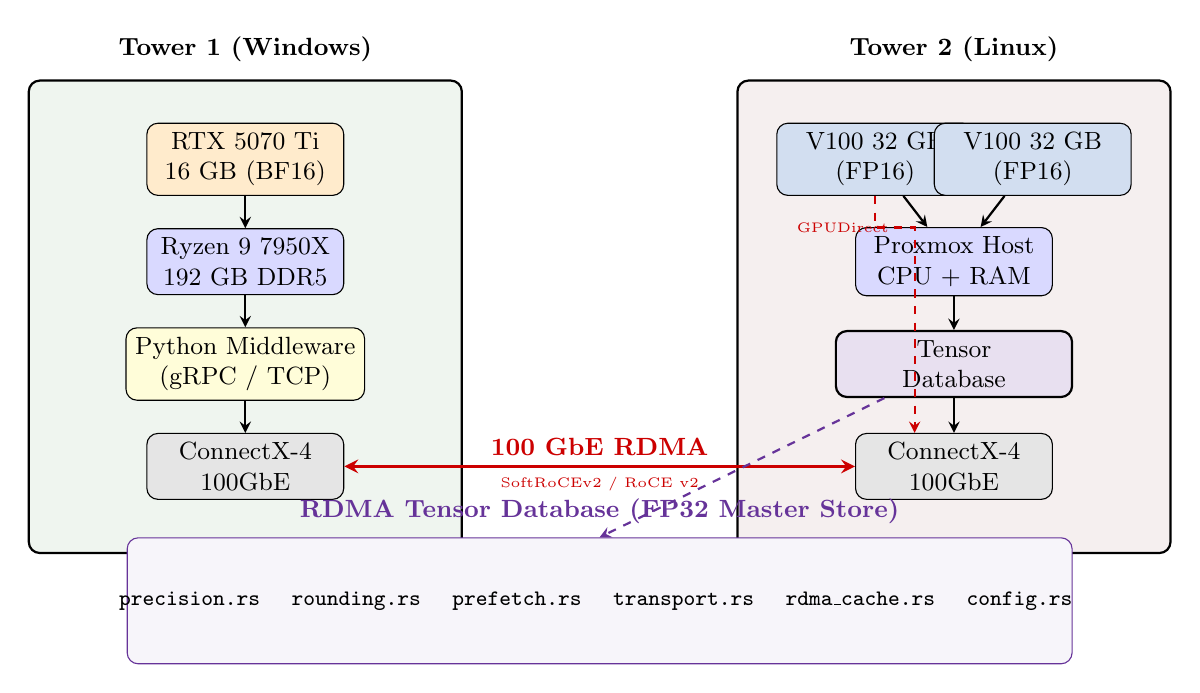
\begin{tikzpicture}[
    node distance=0.6cm and 1.5cm,
    box/.style={rectangle, draw, rounded corners, minimum width=2.5cm, minimum height=0.8cm, align=center, font=\small},
    tower/.style={rectangle, draw, thick, rounded corners, minimum width=5.5cm, minimum height=6cm, align=center},
    db/.style={rectangle, draw, thick, rounded corners, fill=dbpurple!15, minimum width=3cm, minimum height=0.8cm, align=center, font=\small},
    link/.style={<->, >=stealth, very thick},
    arrow/.style={->, >=stealth, thick},
    label/.style={font=\footnotesize}
]

% Tower 1
\node[tower, fill=tower1color!8] (t1) at (-4.5, 0) {};
\node[above=0.1cm of t1.north, font=\small\bfseries] {Tower 1 (Windows)};

\node[box, fill=cudaorange!20] (gpu1) at (-4.5, 2) {RTX 5070 Ti\\16 GB (BF16)};
\node[box, fill=blue!15] (cpu1) at (-4.5, 0.7) {Ryzen 9 7950X\\192 GB DDR5};
\node[box, fill=yellow!15] (mid1) at (-4.5, -0.6) {Python Middleware\\(gRPC / TCP)};
\node[box, fill=gray!20] (nic1) at (-4.5, -1.9) {ConnectX-4\\100GbE};

\draw[arrow] (gpu1) -- (cpu1);
\draw[arrow] (cpu1) -- (mid1);
\draw[arrow] (mid1) -- (nic1);

% Tower 2
\node[tower, fill=tower2color!8] (t2) at (4.5, 0) {};
\node[above=0.1cm of t2.north, font=\small\bfseries] {Tower 2 (Linux)};

\node[box, fill=v100blue!20] (gpu2a) at (3.5, 2) {V100 32 GB\\(FP16)};
\node[box, fill=v100blue!20] (gpu2b) at (5.5, 2) {V100 32 GB\\(FP16)};
\node[box, fill=blue!15] (cpu2) at (4.5, 0.7) {Proxmox Host\\CPU + RAM};
\node[db] (neu) at (4.5, -0.6) {Tensor\\Database};
\node[box, fill=gray!20] (nic2) at (4.5, -1.9) {ConnectX-4\\100GbE};

\draw[arrow] (gpu2a) -- (cpu2);
\draw[arrow] (gpu2b) -- (cpu2);
\draw[arrow] (cpu2) -- (neu);
\draw[arrow] (neu) -- (nic2);

% GPUDirect RDMA annotation
\draw[arrow, dashed, rdmared] (gpu2a.south) -- ++(0, -0.4) -| ($(nic2.north)-(0.5,0)$) node[pos=0.3, left, font=\tiny\color{rdmared}] {GPUDirect};

% 100GbE Link
\draw[link, rdmared] (nic1.east) -- (nic2.west) node[midway, above, font=\small\bfseries] {100 GbE RDMA} node[midway, below, font=\tiny] {SoftRoCEv2 / RoCE v2};

% Tensor Database detail
\node[draw=dbpurple, fill=dbpurple!5, rounded corners, below=2.8cm of $(t1)!0.5!(t2)$, minimum width=12cm, minimum height=1.6cm, align=center] (detail) {};
\node[above=0.05cm of detail.north, font=\small\bfseries\color{dbpurple}] {RDMA Tensor Database (FP32 Master Store)};
\node[font=\footnotesize, align=center] at (detail.center) {
    \texttt{precision.rs} \quad \texttt{rounding.rs} \quad \texttt{prefetch.rs} \quad \texttt{transport.rs} \quad \texttt{rdma\_cache.rs} \quad \texttt{config.rs}
};

\draw[arrow, dbpurple, dashed] (neu) -- (detail.north);

\end{tikzpicture}
\caption{Two-tower system architecture. The tensor database's \texttt{tensor\_rdma} crate runs on Tower~2, serving as the centralized FP32 master weight store. Tower~1 accesses tensors via gRPC/TCP fallback; Tower~2's V100s access them via GPUDirect RDMA through \texttt{nvidia-peermem}.}
\label{fig:system-arch}
\end{figure}

\subsection{Precision Pipeline}

The core challenge is that FP16 (used by V100 Tensor Cores) has 5~exponent bits and 10~mantissa bits, giving a representable range of $[5.96 \times 10^{-8},\; 65504]$. During training, gradient values routinely fall outside this range, causing overflow (gradients $> 65504$ become \texttt{inf}) and underflow (gradients $< 6 \times 10^{-8}$ become zero). BF16 shares FP32's 8~exponent bits, matching its dynamic range of $[1.18 \times 10^{-38},\; 3.4 \times 10^{38}]$, but is unavailable on V100.

\begin{table}[htbp]
\centering
\caption{Floating-point format comparison for LLM training}
\label{tab:fp-comparison}
\begin{tabular}{@{}lccccl@{}}
\toprule
\textbf{Format} & \textbf{Exponent} & \textbf{Mantissa} & \textbf{Range} & \textbf{Bytes} & \textbf{GPU Support} \\
\midrule
FP32 & 8 & 23 & $\pm 3.4 \times 10^{38}$ & 4 & All \\
BF16 & 8 & 7 & $\pm 3.4 \times 10^{38}$ & 2 & Ampere+, not V100 \\
FP16 & 5 & 10 & $\pm 6.5 \times 10^{4}$ & 2 & All (Tensor Cores) \\
MXFP4 & 2 & 1 & $\pm 6$ & 0.5 & Blackwell \\
\bottomrule
\end{tabular}
\end{table}

The critical observation is that BF16 and FP32 share the same exponent width (8 bits), giving BF16 the full FP32 dynamic range at half the memory. FP16's 5-bit exponent limits its range to $6.5 \times 10^4$, which is routinely exceeded during training. Loss scaling partially mitigates this but adds implementation complexity and can mask genuine numerical issues.

The RDMA Tensor Cache resolves this through a three-stage precision pipeline:

\begin{figure}[htbp]
\centering
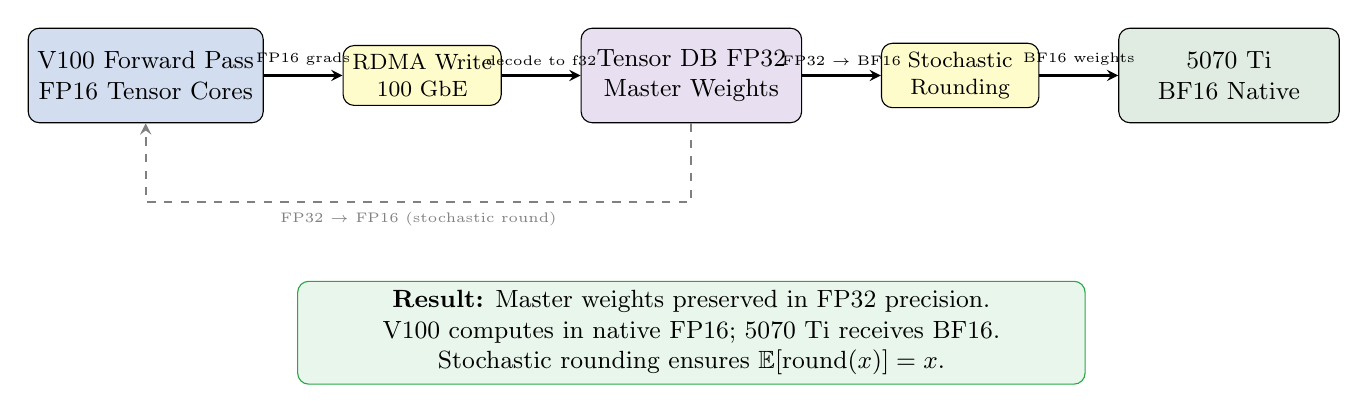
\begin{tikzpicture}[
    node distance=0.5cm and 1.2cm,
    stage/.style={rectangle, draw, rounded corners, minimum width=2.8cm, minimum height=1.2cm, align=center, font=\small},
    op/.style={rectangle, draw, rounded corners, fill=yellow!20, minimum width=2cm, minimum height=0.6cm, align=center, font=\footnotesize},
    arrow/.style={->, >=stealth, thick},
    label/.style={font=\footnotesize}
]

% V100 compute
\node[stage, fill=v100blue!20] (v100) {V100 Forward Pass\\FP16 Tensor Cores};

% RDMA transfer
\node[op, right=1cm of v100] (rdma1) {RDMA Write\\100 GbE};

% FP32 master
\node[stage, fill=dbpurple!15, right=1cm of rdma1] (master) {Tensor DB FP32\\Master Weights};

% Stochastic round
\node[op, right=1cm of master] (sr) {Stochastic\\Rounding};

% BF16 output
\node[stage, fill=tower1color!15, right=1cm of sr] (bf16) {5070 Ti\\BF16 Native};

% Arrows
\draw[arrow] (v100) -- node[above, font=\tiny] {FP16 grads} (rdma1);
\draw[arrow] (rdma1) -- node[above, font=\tiny] {decode to f32} (master);
\draw[arrow] (master) -- node[above, font=\tiny] {FP32 $\to$ BF16} (sr);
\draw[arrow] (sr) -- node[above, font=\tiny] {BF16 weights} (bf16);

% Feedback loop
\draw[arrow, dashed, gray] (master.south) -- ++(0,-1) -| (v100.south) node[pos=0.25, below, font=\tiny] {FP32 $\to$ FP16 (stochastic round)};

% Mixed precision annotation
\node[draw=solutiongreen, fill=solutiongreen!10, rounded corners, below=2cm of master, minimum width=10cm, align=center, font=\small] (benefit) {
    \textbf{Result:} Master weights preserved in FP32 precision.\\
    V100 computes in native FP16; 5070~Ti receives BF16.\\
    Stochastic rounding ensures $\mathbb{E}[\text{round}(x)] = x$.
};

\end{tikzpicture}
\caption{Precision pipeline. Gradients computed in V100 FP16 are accumulated into FP32 master weights stored in the tensor database. Stochastic rounding converts to device-native precision for each GPU.}
\label{fig:precision-pipeline}
\end{figure}

\subsection{Stochastic Rounding}
\label{sec:stochastic-rounding}

Standard rounding (round-to-nearest-even) introduces a systematic bias when converting FP32 values to reduced precision: values exactly between two representable numbers always round to the even option, causing certain gradient directions to be preferred. Stochastic rounding eliminates this bias by making the rounding direction probabilistic.

For an FP32 value $x$ being rounded to a lower-precision format with adjacent representable values $\lfloor x \rfloor$ and $\lceil x \rceil$:
\begin{equation}
\label{eq:stochastic-round}
    P(\text{round up}) = \frac{x - \lfloor x \rfloor_{\text{fp16}}}{\lceil x \rceil_{\text{fp16}} - \lfloor x \rfloor_{\text{fp16}}}
\end{equation}
This gives the unbiasedness property:
\begin{equation}
    \mathbb{E}[\text{round}(x)] = \lfloor x \rfloor \cdot (1 - P) + \lceil x \rceil \cdot P = x
\end{equation}
which ensures that gradient accumulation over many steps converges to the correct value despite precision loss in individual steps~\cite{micikevicius2018mixed}.

In the \texttt{tensor\_rdma} crate, stochastic rounding is implemented in \texttt{rounding.rs} using the \texttt{half} crate for FP16/BF16 manipulation and \texttt{rand} for probability generation. The core function, \texttt{stochastic\_round\_f32\_to\_f16}, takes an FP32 value and a random number generator as inputs and returns an FP16 result. It first truncates the input to the nearest lower FP16 representable value (the ``floor'') and converts that floor back to FP32 to measure the truncation error. If the original value is exactly representable in FP16 (the difference falls within machine epsilon), the floor is returned directly. Otherwise, the function computes the next higher representable FP16 value (the ``ceiling'') using bit-level manipulation via a \texttt{next\_fp16} helper. It then calculates the fractional position of the original FP32 value between the floor and ceiling, and uses a uniform random draw to decide the rounding direction: if the random value falls below the fraction, the result rounds up to the ceiling; otherwise it rounds down to the floor. This procedure guarantees that the expected value of the rounded output equals the original FP32 input, eliminating the systematic directional bias inherent in deterministic rounding during gradient accumulation.

\subsection{Centralized KV Cache}

The MLA/MQA duplication problem identified in Section~\ref{sec:mla-problem} is resolved by storing the KV cache in the tensor database's \texttt{RdmaTensorCache}, keyed by layer index and sequence position. Each TP rank issues one-sided RDMA reads to fetch the KV entries it needs for its attention head shard, rather than maintaining a local copy.

The RDMA read pattern for KV cache access is:
\begin{enumerate}
    \item Prefetch engine predicts which layer/position entries will be needed next based on the current decoding step.
    \item Transport layer issues RDMA Read to the tensor database's registered buffer for the predicted entries.
    \item Attention computation proceeds on local GPU memory with the fetched KV data.
    \item New KV entries generated during decoding are written back via RDMA Write.
\end{enumerate}

For a model with $L$ layers and context length $C$, this reduces total KV memory across TP ranks from $\text{TP} \times 2LC \cdot d_{\text{kv}}$ to $2LC \cdot d_{\text{kv}} + \text{TP} \times \text{prefetch\_buffer}$. The prefetch buffer is typically 3--5 layers deep, a small fraction of the total cache.

%=============================================================================
\section{Tensor Database Architecture}
\label{sec:database-architecture}
%=============================================================================

The \texttt{tensor\_rdma} crate~\cite{scuffedrdma-repo} is a workspace member in the tensor database runtime. It depends on \texttt{tensor\_store} for local key-value storage and \texttt{tensor\_compress} for delta encoding. \Cref{fig:crate-deps} shows the dependency structure.

\begin{figure}[htbp]
\centering
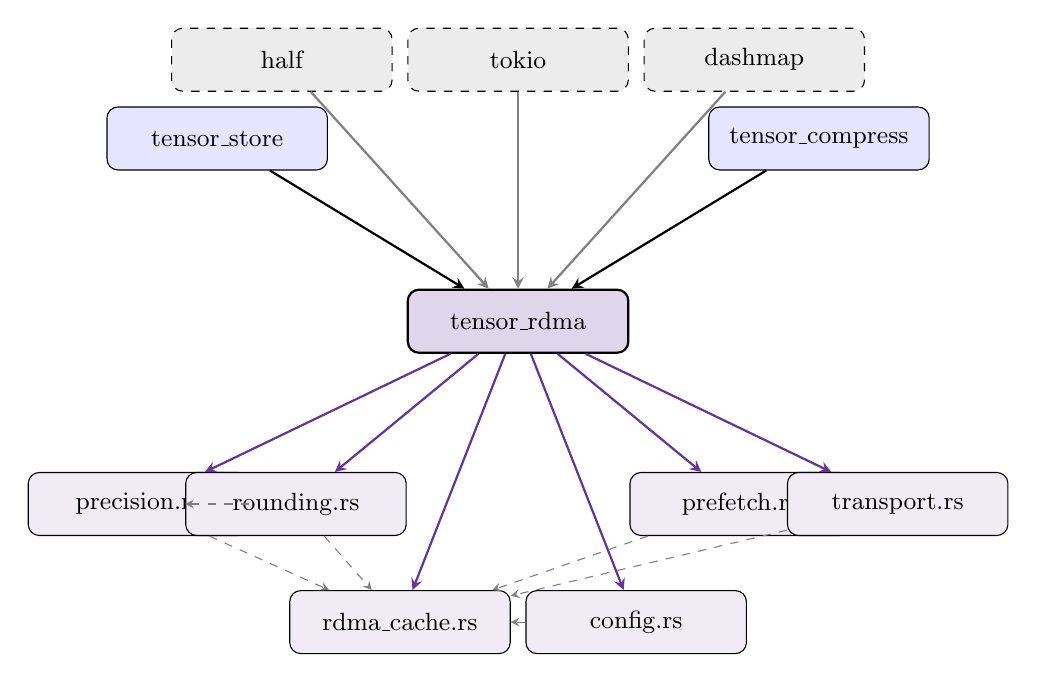
\begin{tikzpicture}[
    node distance=1.2cm and 1.5cm,
    crate/.style={rectangle, draw, rounded corners, minimum width=2.8cm, minimum height=0.8cm, align=center, font=\small},
    rdma/.style={crate, fill=dbpurple!20, thick},
    dep/.style={crate, fill=blue!10},
    ext/.style={crate, fill=gray!15, dashed},
    arrow/.style={->, >=stealth, thick}
]

% tensor_rdma (center)
\node[rdma] (rdma) {tensor\_rdma};

% Internal dependencies
\node[dep, above left=1.5cm and 1cm of rdma] (store) {tensor\_store};
\node[dep, above right=1.5cm and 1cm of rdma] (compress) {tensor\_compress};

% Modules within tensor_rdma
\node[crate, fill=dbpurple!10, below left=1.5cm and 2cm of rdma] (precision) {precision.rs};
\node[crate, fill=dbpurple!10, below left=1.5cm and 0cm of rdma] (rounding) {rounding.rs};
\node[crate, fill=dbpurple!10, below right=1.5cm and 0cm of rdma] (prefetch) {prefetch.rs};
\node[crate, fill=dbpurple!10, below right=1.5cm and 2cm of rdma] (transport) {transport.rs};
\node[crate, fill=dbpurple!10, below=3cm of rdma, xshift=-1.5cm] (cache) {rdma\_cache.rs};
\node[crate, fill=dbpurple!10, below=3cm of rdma, xshift=1.5cm] (config) {config.rs};

% External crates
\node[ext, above=2.5cm of rdma, xshift=-3cm] (half) {half};
\node[ext, above=2.5cm of rdma, xshift=0cm] (tokio) {tokio};
\node[ext, above=2.5cm of rdma, xshift=3cm] (dashmap) {dashmap};

% Arrows: external -> tensor_rdma
\draw[arrow, gray] (half) -- (rdma);
\draw[arrow, gray] (tokio) -- (rdma);
\draw[arrow, gray] (dashmap) -- (rdma);

% Arrows: internal deps
\draw[arrow] (store) -- (rdma);
\draw[arrow] (compress) -- (rdma);

% Arrows: modules
\draw[arrow, dbpurple] (rdma) -- (precision);
\draw[arrow, dbpurple] (rdma) -- (rounding);
\draw[arrow, dbpurple] (rdma) -- (prefetch);
\draw[arrow, dbpurple] (rdma) -- (transport);
\draw[arrow, dbpurple] (rdma) -- (cache);
\draw[arrow, dbpurple] (rdma) -- (config);

% Module inter-deps
\draw[arrow, dashed, gray, thin] (precision) -- (rounding);
\draw[arrow, dashed, gray, thin] (precision) -- (cache);
\draw[arrow, dashed, gray, thin] (rounding) -- (cache);
\draw[arrow, dashed, gray, thin] (prefetch) -- (cache);
\draw[arrow, dashed, gray, thin] (transport) -- (cache);
\draw[arrow, dashed, gray, thin] (config) -- (cache);

\end{tikzpicture}
\caption{Tensor database \texttt{tensor\_rdma} crate dependency graph. The crate depends on \texttt{tensor\_store} for local caching and \texttt{tensor\_compress} for delta encoding. Six internal modules implement the RDMA Tensor Cache.}
\label{fig:crate-deps}
\end{figure}

\subsection{Module Mapping}

\Cref{tab:module-mapping} maps thesis concepts to their Rust implementations.

\begin{table}[htbp]
\centering
\caption{Thesis concepts mapped to \texttt{tensor\_rdma} modules}
\label{tab:module-mapping}
\begin{tabular}{@{}llp{6cm}@{}}
\toprule
\textbf{Thesis Concept} & \textbf{Module} & \textbf{Key Types / Functions} \\
\midrule
Precision management & \texttt{precision.rs} & \texttt{PrecisionFormat} (FP16, BF16, FP32, MXFP4), \texttt{DeviceCapability}, \texttt{PrecisionRouter}, \texttt{convert\_precision} \\
Stochastic rounding & \texttt{rounding.rs} & \texttt{stochastic\_round\_f32\_to\_f16}, \texttt{apply\_adam\_update}, \texttt{apply\_gradient\_batch} \\
Predictive prefetching & \texttt{prefetch.rs} & \texttt{PrefetchEngine}, \texttt{AccessPattern} (Sequential, Strided, LayerSweep, Random), \texttt{classify\_pattern} \\
RDMA transport & \texttt{transport.rs} & \texttt{RdmaTransport} trait, \texttt{MemoryTransport}, \texttt{TcpFallbackTransport}, \texttt{BufferHandle}, \texttt{RemoteAddr} \\
Tensor cache & \texttt{rdma\_cache.rs} & \texttt{RdmaTensorCache<T>}, \texttt{put\_tensor}, \texttt{get\_tensor}, \texttt{apply\_gradient}, \texttt{get\_wire\_tensor} \\
Configuration & \texttt{config.rs} & \texttt{RdmaCacheConfig}, \texttt{PrefetchStrategy}, \texttt{TransportConfig}, presets: \texttt{v100\_preset}, \texttt{heterogeneous\_preset} \\
\bottomrule
\end{tabular}
\end{table}

\subsection{Device Capability Model}

The \texttt{DeviceCapability} struct encodes what each GPU supports, and the \texttt{PrecisionRouter} uses these capabilities to select wire formats. For our hardware, two device capability presets are defined. The V100 preset (\texttt{DeviceCapability::v100\_32gb()}) describes the Tesla V100 32\,GB as supporting FP16 and FP32 formats with FP16 as the native compute precision, 32\,GB of VRAM, and GPUDirect RDMA enabled. The RTX 5070~Ti preset (\texttt{DeviceCapability::rtx5070ti()}) describes the consumer GPU as supporting FP16, BF16, and FP32 with BF16 as the native compute precision, 16\,GB of VRAM, and GPUDirect RDMA disabled (since Windows lacks kernel-level RDMA support).

The \texttt{PrecisionRouter::common\_format()} method determines the lowest common denominator: for V100 + 5070~Ti, this is FP16 (since V100 lacks BF16). However, the cache stores in FP32 and converts per-device, avoiding the precision ceiling that a common format would impose.

\subsection{Transport Abstraction}

The \texttt{RdmaTransport} trait defines four core operations modeled on RDMA verbs semantics:

\begin{enumerate}
    \item \texttt{register\_buffer}: Analogous to \texttt{ibv\_reg\_mr}. Pins memory and returns a \texttt{BufferHandle} with a remote key.
    \item \texttt{deregister\_buffer}: Releases the memory registration.
    \item \texttt{rdma\_write}: One-sided write to a remote buffer at a specified offset. No notification to the remote CPU.
    \item \texttt{rdma\_read}: One-sided read from a remote buffer. Data is pulled without remote CPU involvement.
\end{enumerate}

Three implementations exist: \texttt{MemoryTransport} for unit testing (shared \texttt{HashMap} simulating RDMA), \texttt{TcpFallbackTransport} for Windows (Tower~1), and the planned \texttt{SoftRoceTransport} for Linux (Tower~2, feature-gated behind \texttt{rdma-core}).

%=============================================================================
\section{Experimental Design: Three Pillars}
\label{sec:experiments}
%=============================================================================

We structure validation around three experimental pillars, each targeting a distinct aspect of the RDMA Tensor Cache.

\subsection{Pillar 1: Precision Switching Overhead}

\textbf{Hypothesis:} Stochastic rounding adds less than 5\% overhead compared to deterministic truncation, while eliminating the gradient bias that causes training divergence.

\textbf{Methodology:}
\begin{enumerate}
    \item Generate synthetic gradient tensors of varying sizes ($10^3$ to $10^8$ elements) spanning the FP16 representable range.
    \item Measure wall-clock time for FP16 $\to$ FP32 decode, FP32 weight update, and FP32 $\to$ FP16 stochastic round.
    \item Compare against deterministic round-to-nearest on the same tensors.
    \item Compute bias: $\text{Bias} = \frac{1}{N}\sum_{i=1}^{N} (\text{round}(x_i) - x_i)$ over $10^6$ samples.
\end{enumerate}

\textbf{Metrics:}
\begin{itemize}
    \item Conversion throughput (GB/s) for each direction: FP16$\leftrightarrow$FP32, FP32$\leftrightarrow$BF16
    \item Statistical bias magnitude (should be $< 10^{-6}$ for stochastic, $> 10^{-4}$ for deterministic)
    \item Overhead ratio: $T_{\text{stochastic}} / T_{\text{deterministic}}$
\end{itemize}

\subsection{Pillar 2: Prefetching Effectiveness}

\textbf{Hypothesis:} The adaptive prefetch engine achieves $>$90\% hit rate for sequential inference workloads and $>$70\% for fine-tuning workloads, hiding RDMA latency for the majority of tensor accesses.

\begin{figure}[htbp]
\centering
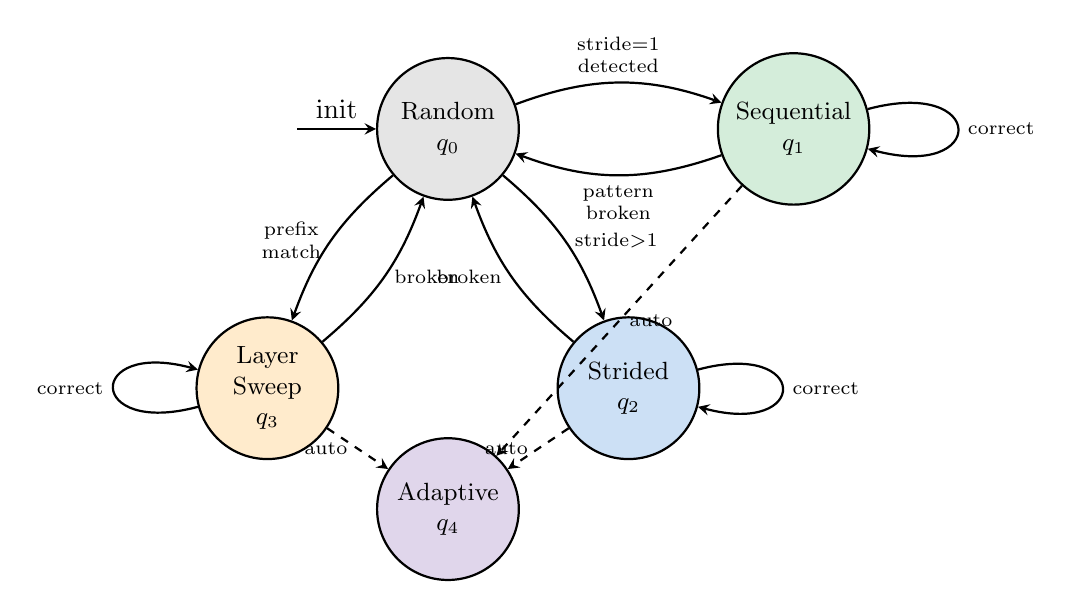
\begin{tikzpicture}[
    node distance=1.8cm,
    state/.style={circle, draw, thick, minimum size=1.8cm, align=center, font=\small},
    seq/.style={state, fill=solutiongreen!20},
    str/.style={state, fill=ucxblue!20},
    lsw/.style={state, fill=cudaorange!20},
    adp/.style={state, fill=dbpurple!20},
    rnd/.style={state, fill=gray!20},
    arrow/.style={->, >=stealth, thick},
    label/.style={font=\scriptsize, align=center}
]

% States
\node[rnd] (random) {Random\\$q_0$};
\node[seq, right=2.5cm of random] (seq) {Sequential\\$q_1$};
\node[str, below right=2cm and 1cm of random] (str) {Strided\\$q_2$};
\node[lsw, below left=2cm and 1cm of random] (lsw) {Layer\\Sweep\\$q_3$};
\node[adp, below=3cm of random] (adp) {Adaptive\\$q_4$};

% Initial
\draw[arrow] ($(random.west)+(-1,0)$) -- (random) node[midway, above] {init};

% Transitions
\draw[arrow, bend left=20] (random) to node[above, label] {stride=1\\detected} (seq);
\draw[arrow, bend left=20] (seq) to node[below, label] {pattern\\broken} (random);

\draw[arrow, bend left=15] (random) to node[right, label] {stride$>$1} (str);
\draw[arrow, bend left=15] (str) to node[left, label] {broken} (random);

\draw[arrow, bend right=15] (random) to node[left, label] {prefix\\match} (lsw);
\draw[arrow, bend right=15] (lsw) to node[right, label] {broken} (random);

% Adaptive transitions
\draw[arrow, dashed] (seq) to node[right, label] {auto} (adp);
\draw[arrow, dashed] (str) to node[left, label] {auto} (adp);
\draw[arrow, dashed] (lsw) to node[left, label] {auto} (adp);

% Self loops
\draw[arrow] (seq) to[loop right] node[label] {correct} (seq);
\draw[arrow] (str) to[loop right] node[label] {correct} (str);
\draw[arrow] (lsw) to[loop left] node[label] {correct} (lsw);

\end{tikzpicture}
\caption{Prefetch engine state machine. The \texttt{Adaptive} strategy delegates to the detected pattern. State transitions occur when the \texttt{classify\_pattern} function analyzes the access history buffer (1024~entries).}
\label{fig:prefetch-fsm}
\end{figure}

\textbf{Methodology:}
\begin{enumerate}
    \item Trace tensor access patterns during Llama-7B inference on a single V100 (sequential layer-by-layer).
    \item Trace access patterns during LoRA fine-tuning (forward sequential, backward reverse, optimizer random).
    \item Replay traces through the prefetch engine with varying depths (1, 3, 5, 10).
    \item Measure hit rate: fraction of accesses where the tensor was already prefetched.
\end{enumerate}

\textbf{Metrics:}
\begin{itemize}
    \item Prefetch hit rate by strategy (Sequential, Strided, LayerSweep, Adaptive)
    \item Latency breakdown: hit path ($<$1~$\mu$s local lookup) vs.\ miss path (190~$\mu$s SoftRoCE / 2~$\mu$s hardware RoCE)
    \item Wasted prefetches: tensors prefetched but never used (bandwidth waste)
\end{itemize}

\subsection{Pillar 3: Adaptive Quantization}

\textbf{Hypothesis:} MXFP4 quantization~\cite{rouhani2023mxfp4} achieves 4$\times$ bandwidth reduction with less than 1\% accuracy loss for inference-time KV cache transfers, and stochastic rounding preserves gradient quality under 2$\times$ FP16 bandwidth reduction.

\textbf{Methodology:}
\begin{enumerate}
    \item Measure inference quality (perplexity on WikiText-2) with KV cache stored in FP32, FP16, BF16, and MXFP4.
    \item Measure training convergence (loss curve) with gradients transferred in FP32, FP16 (deterministic), and FP16 (stochastic).
    \item Profile 100GbE utilization under each precision configuration.
\end{enumerate}

\textbf{Metrics:}
\begin{itemize}
    \item Perplexity delta: $\Delta \text{PPL} = \text{PPL}_{\text{quantized}} - \text{PPL}_{\text{FP32}}$
    \item Bandwidth savings: bytes transferred per training step
    \item Convergence rate: steps to reach target loss
\end{itemize}

\subsection{Target Performance Summary}

\begin{table}[htbp]
\centering
\caption{Target performance metrics across all three pillars}
\label{tab:target-metrics}
\begin{tabular}{@{}llcc@{}}
\toprule
\textbf{Pillar} & \textbf{Metric} & \textbf{Baseline} & \textbf{Target} \\
\midrule
\multirow{3}{*}{Precision} & Stochastic round overhead & -- & $< 5\%$ \\
 & Bias (stochastic) & -- & $< 10^{-6}$ \\
 & Conversion throughput & -- & $> 50$ GB/s \\
\midrule
\multirow{3}{*}{Prefetching} & Hit rate (inference) & 0\% & $> 90\%$ \\
 & Hit rate (fine-tuning) & 0\% & $> 70\%$ \\
 & Wasted prefetch ratio & -- & $< 15\%$ \\
\midrule
\multirow{3}{*}{Quantization} & $\Delta$PPL (FP16 KV) & FP32 & $< 0.1$ \\
 & $\Delta$PPL (MXFP4 KV) & FP32 & $< 0.5$ \\
 & Bandwidth reduction & 1$\times$ & $2$--$4\times$ \\
\bottomrule
\end{tabular}
\end{table}

The three pillars are designed to be independently measurable but collectively demonstrate the viability of the RDMA Tensor Cache for production heterogeneous clusters. Pillar~1 validates the precision management layer in isolation; Pillar~2 validates the prefetch engine's ability to hide network latency; Pillar~3 demonstrates end-to-end quality preservation under aggressive bandwidth reduction.

\subsection{Workload Specifications}

The experimental workloads target models that exercise the full precision pipeline:

\begin{enumerate}
    \item \textbf{Llama 2 7B (inference):} Sequential layer-by-layer access pattern. KV cache grows linearly with generated tokens. Tests Pillar~2 (sequential prefetch) and Pillar~3 (KV cache quantization).

    \item \textbf{Mistral 7B with Sliding Window (inference):} Strided access pattern due to sliding window attention. KV cache has fixed maximum size. Tests Pillar~2 (strided prefetch detection).

    \item \textbf{DeepSeek-V2 Lite (inference):} MLA attention with compressed latent representation. Single KV head, directly exercises the centralized KV cache design from Section~\ref{sec:mla-problem}.

    \item \textbf{Llama 2 7B LoRA (fine-tuning):} Forward (sequential), backward (reverse sequential), optimizer (random access). Tests all three prefetch strategies and the full gradient$\to$master weight$\to$device weight pipeline.
\end{enumerate}

%=============================================================================
\section{Multistage Fine-Tuning and SAE Feature Steering}
\label{sec:finetuning-sae}
%=============================================================================

We investigate two approaches to adapting LLMs on our heterogeneous cluster: traditional gradient-based fine-tuning with the RDMA Tensor Cache, and SAE-based feature steering as a gradient-free alternative.

\subsection{Traditional Fine-Tuning Pipeline}

The heterogeneous training pipeline assigns roles based on GPU capabilities:

\begin{itemize}
    \item \textbf{V100 pair (Tower 2):} Forward and backward passes in FP16 Tensor Cores. Gradients are produced in FP16 and transferred to the tensor database via RDMA.
    \item \textbf{Tensor Database (Tower 2 host):} Accumulates gradients into FP32 master weights. Applies optimizer updates (Adam) in full precision.
    \item \textbf{5070 Ti (Tower 1):} Receives BF16 weights via TCP/gRPC for inference validation during training. Can also run the optimizer in BF16 for tasks where BF16 dynamic range is sufficient.
\end{itemize}

This architecture mirrors the Hetis system~\cite{hetis2024}, which demonstrated 2.25$\times$ throughput improvement by assigning distinct stages of the training pipeline to different GPU types. In Hetis, heterogeneous GPUs handle prefill and decode stages separately. We adapt this idea to separate compute (V100 FP16) from precision management (Tensor DB FP32) and validation (5070~Ti BF16).

\subsection{Sparse Auto-Encoder Feature Steering}
\label{sec:sae}

Sparse Auto-Encoders (SAEs) offer an alternative to gradient-based fine-tuning for modifying model behavior. Instead of adjusting model weights through backpropagation, SAEs decompose model activations into interpretable features that can be directly manipulated~\cite{cunningham2023sae}.

An SAE decomposes a model's internal activation vector $\mathbf{a} \in \mathbb{R}^d$ into a sparse feature vector $\mathbf{f} \in \mathbb{R}^D$ where $D \gg d$:
\begin{equation}
    \mathbf{f} = \text{ReLU}(W_{\text{enc}} \cdot \mathbf{a} + \mathbf{b}_{\text{enc}})
\end{equation}
\begin{equation}
    \hat{\mathbf{a}} = W_{\text{dec}} \cdot \mathbf{f} + \mathbf{b}_{\text{dec}}
\end{equation}
The key property is that $\mathbf{f}$ is sparse: only $k \ll D$ features are active for any given input. Cunningham et al.~\cite{cunningham2023sae} showed that these features correspond to interpretable concepts (e.g., ``mentions of the Eiffel Tower,'' ``Python code patterns,'' ``formal writing style'').

\subsubsection{Feature Steering}

Given a trained SAE, model behavior can be modified by clamping or scaling specific features. To steer the model toward producing outputs related to feature $i$:
\begin{equation}
    \mathbf{f}'_i = \alpha \cdot \mathbf{f}_{\max,i}
\end{equation}
where $\alpha$ controls the steering strength and $\mathbf{f}_{\max,i}$ is the maximum activation observed for feature $i$ during training. The modified activation is then:
\begin{equation}
    \mathbf{a}' = W_{\text{dec}} \cdot \mathbf{f}' + \mathbf{b}_{\text{dec}}
\end{equation}

This modification is applied at inference time with no gradient computation, no backward pass, and no weight updates. The Eiffel Tower Llama demo~\cite{eiffel-tower-llama} demonstrates this: clamping the ``Eiffel Tower'' feature causes Llama to mention the Eiffel Tower in every response regardless of the prompt.

\subsubsection{Mapping to the Tensor Database}

SAE feature vectors are a natural fit for the tensor database's \texttt{SparseVector} type, which stores only non-zero indices and values. A typical SAE feature vector has 65,536 dimensions but only approximately 50 active features: the dense representation requires $65{,}536 \times 4 = 256$\,KB, while the \texttt{SparseVector} stores only the active index--value pairs, consuming roughly $50 \times (4 + 4) = 400$\,bytes---a 51$\times$ compression ratio. These sparse vectors are stored in the tensor database under descriptive keys (e.g., \texttt{sae:layer\_12:eiffel\_tower}) and made available for RDMA access by both towers. A single feature vector at approximately 400~bytes fits well within a single RDMA read, far below the network MTU.

OpenAI's work on scaling SAEs~\cite{openai-sae-scaling} and the HuggingFace SAE collection~\cite{sae-collection} provide pre-trained SAEs for several open-weight models. These can be loaded into the tensor database and served to both towers for inference-time steering.

\subsubsection{Advantages over Gradient-Based Fine-Tuning}

\begin{table}[htbp]
\centering
\caption{Comparison of fine-tuning approaches for our hardware}
\label{tab:finetuning-comparison}
\begin{tabular}{@{}lcc@{}}
\toprule
\textbf{Property} & \textbf{Gradient-Based (LoRA)} & \textbf{SAE Steering} \\
\midrule
Requires backward pass & Yes & No \\
GPU memory for optimizer & 2--3$\times$ model size & Zero \\
Training time & Hours to days & Seconds (feature lookup) \\
Precision sensitivity & High (requires FP32 master) & Low (sparse vector ops) \\
Cross-tower RDMA traffic & Gradients per step & Feature vectors once \\
Reversibility & Requires separate checkpoint & Immediate (set $\alpha = 0$) \\
Interpretability & Opaque weight deltas & Named features \\
\bottomrule
\end{tabular}
\end{table}

SAE steering does not replace fine-tuning for all tasks. It cannot learn genuinely new capabilities, only amplify or suppress existing features. However, for behavioral adaptation (style, tone, topic focus) it eliminates the entire precision management pipeline and reduces RDMA traffic to a single sparse vector read.

%=============================================================================
\section{Python Prototype}
\label{sec:python-prototype}
%=============================================================================

The Python prototype bridges the \texttt{tensor\_rdma} Rust crate with vLLM's distributed inference engine. It follows the middleware architecture established in earlier work on the ScuffedRDMA communication layer and extends it with RDMA-native connectors.

\subsection{Architecture}

\begin{lstlisting}[language=Python, caption={RDMA Tensor Cache middleware extension}]
class RDMATensorCacheMiddleware:
    """Extends the ScuffedRDMA middleware with RDMA tensor database access."""

    def __init__(self, config: MiddlewareConfig):
        self.transport = self._init_transport(config)
        self.db_client = DatabaseClient(
            host=config.db_host,  # 192.168.2.111
            port=config.db_port,  # 4791
        )
        self.precision_router = PrecisionRouter(config.devices)

    def get_tensor(self, key: str, device: DeviceCapability) -> torch.Tensor:
        """Fetch tensor from the tensor database with automatic precision conversion."""
        wire_format = self.precision_router.optimal_wire_format(device)
        raw = self.db_client.rdma_read(key)
        return self._decode_to_torch(raw, wire_format, device)

    def put_gradient(self, key: str, gradient: torch.Tensor,
                     source_device: DeviceCapability) -> None:
        """Send gradient to the tensor database for FP32 master weight update."""
        wire_data = self._encode_from_torch(gradient, source_device)
        self.db_client.rdma_write(key, wire_data)

    def get_kv_cache(self, layer_idx: int, seq_positions: List[int]
                     ) -> torch.Tensor:
        """Fetch KV cache entries from the centralized tensor database."""
        keys = [f"kv:layer_{layer_idx}:pos_{p}" for p in seq_positions]
        return self.db_client.batch_read(keys)
\end{lstlisting}

\subsection{vLLM Connector}

The connector follows vLLM's existing patterns for distributed KV cache management. vLLM supports pluggable connectors (MooncakeConnector~\cite{mooncake2024}, NixlConnector~\cite{nixl}) through its transfer engine interface. Our connector implements the same interface:

\begin{lstlisting}[language=Python, caption={vLLM RDMA connector skeleton}]
class RDMAKVConnector:
    """vLLM KV cache connector backed by the RDMA Tensor Database."""

    def __init__(self, vllm_config, role: str):
        self.role = role  # "prefill" or "decode"
        self.middleware = RDMATensorCacheMiddleware(
            MiddlewareConfig.from_vllm(vllm_config)
        )

    def send_kv_caches_and_hidden_states(
        self, model_executable, model_input, kv_caches, hidden_states
    ):
        """Push KV caches to the tensor database after prefill."""
        for layer_idx, kv in enumerate(kv_caches):
            key = f"kv:req_{model_input.request_id}:layer_{layer_idx}"
            self.middleware.db_client.rdma_write(key, kv)

    def recv_kv_caches_and_hidden_states(self, model_executable, model_input):
        """Pull KV caches from the tensor database for decode."""
        kv_caches = []
        for layer_idx in range(model_executable.num_layers):
            key = f"kv:req_{model_input.request_id}:layer_{layer_idx}"
            kv = self.middleware.get_kv_cache(layer_idx, model_input.positions)
            kv_caches.append(kv)
        return kv_caches, None
\end{lstlisting}

%=============================================================================
\section{SoftRoCEv2 Baseline}
\label{sec:softroce}
%=============================================================================

Before deploying hardware RoCE with the ConnectX-4 NICs, we establish a SoftRoCEv2 baseline for Tower~1 $\leftrightarrow$ Tower~2 communication. SoftRoCEv2 implements the RDMA verbs API in software over standard Ethernet, enabling development and debugging of RDMA code paths without specialized hardware configuration.

\subsection{Configuration}

On Tower~2 (Proxmox/Linux), SoftRoCEv2 is configured by loading the \texttt{rdma\_rxe} kernel module and creating an RXE device bound to the physical NIC (\texttt{ens3f0}) using the \texttt{rdma link add} command. After creation, \texttt{rdma link show} confirms that the RXE device is in the ACTIVE state with physical link up over the specified network device. Querying the device with \texttt{ibv\_devinfo} reports it as an InfiniBand transport device with software firmware (version 0.0.0), supporting up to 1024 queue pairs and the maximum possible memory region size. This software RDMA provider exercises the same verbs API as hardware InfiniBand, enabling full development and testing of RDMA code paths.

\subsection{GPUDirect RDMA Setup}

For the V100 GPUs on Tower~2, GPUDirect RDMA provides the most efficient data path. With \texttt{nvidia-peermem} loaded, the RDMA NIC can read/write GPU memory directly. The setup involves loading the \texttt{nvidia-peermem} kernel module and verifying that GPU BAR1 memory is accessible, which for the V100 32\,GB reports a total BAR1 space of 32,768\,MiB. RDMA write bandwidth can then be tested using the \texttt{perftest} suite's \texttt{ib\_write\_bw} tool with the \texttt{-{}-use\_cuda=0} flag to target GPU~0 memory, running in server mode on one end and client mode connecting to the Tower~2 address (192.168.2.111) on the other.

\subsection{Expected Baseline Measurements}

\begin{table}[htbp]
\centering
\caption{Expected SoftRoCEv2 baseline performance (Tower 1 $\leftrightarrow$ Tower 2)}
\label{tab:softroce-baseline}
\begin{tabular}{@{}lccc@{}}
\toprule
\textbf{Metric} & \textbf{SoftRoCEv2} & \textbf{Hardware RoCE (target)} & \textbf{Improvement} \\
\midrule
Latency (1 byte) & $\sim$190 $\mu$s & $\sim$2 $\mu$s & 95$\times$ \\
Bandwidth (large msg) & $\sim$8 Gbps & $\sim$90 Gbps & 11$\times$ \\
CPU overhead & High (software path) & Near-zero (NIC offload) & -- \\
GPUDirect RDMA & Via host bounce & Direct NIC$\to$GPU & -- \\
\bottomrule
\end{tabular}
\end{table}

SoftRoCEv2 exercises the same verbs API as hardware RoCE, so code developed against it requires no changes when transitioning to hardware. The primary limitations are latency (dominated by kernel context switches) and bandwidth (limited by CPU processing of RDMA protocol headers).

\subsection{Benchmark Methodology}

The SoftRoCEv2 baseline will be established using the standard \texttt{perftest} suite and custom tensor transfer benchmarks:

\begin{enumerate}
    \item \textbf{Microbenchmarks (perftest):}
    \begin{itemize}
        \item \texttt{ib\_write\_lat}: RDMA Write latency for message sizes 1~B to 4~MB.
        \item \texttt{ib\_read\_lat}: RDMA Read latency (same range).
        \item \texttt{ib\_write\_bw}: Sustained write bandwidth with 64~KB to 16~MB messages.
        \item \texttt{ib\_read\_bw}: Sustained read bandwidth.
    \end{itemize}

    \item \textbf{Tensor transfer benchmarks:}
    \begin{itemize}
        \item Round-trip latency for gradient tensors of sizes matching common transformer layers (1024$\times$1024, 4096$\times$4096, 8192$\times$8192).
        \item Sustained throughput for streaming weight downloads (simulating model loading via RDMA).
        \item Concurrent transfer scalability: 1, 2, 4, 8 simultaneous QPs.
    \end{itemize}

    \item \textbf{GPUDirect RDMA benchmarks:}
    \begin{itemize}
        \item CPU-staged vs.\ GPUDirect latency and throughput comparison on Tower~2.
        \item GPU memory registration overhead (\texttt{ibv\_reg\_mr} with \texttt{nvidia-peermem}).
        \item Effect of GPU memory allocation strategy (\texttt{cudaMalloc} vs.\ \texttt{cudaMallocManaged}).
    \end{itemize}
\end{enumerate}

These measurements establish the performance envelope for each transport path, informing the prefetch engine's latency estimates and the middleware's transport selection heuristics.

%=============================================================================
\section{UCX/UCC Integration Path}
\label{sec:ucx-ucc}
%=============================================================================

\subsection{UCX Transport Mapping}

The middleware's transport abstraction maps directly to UCX transport layers. \Cref{tab:ucx-mapping} shows the correspondence:

\begin{table}[htbp]
\centering
\caption{Middleware transport mapping to UCX}
\label{tab:ucx-mapping}
\begin{tabular}{@{}lll@{}}
\toprule
\textbf{Middleware Transport} & \textbf{UCX Transport (UCX\_TLS)} & \textbf{Use Case} \\
\midrule
\texttt{TcpFallbackTransport} & \texttt{tcp} & Tower 1 (Windows, no RDMA) \\
\texttt{SoftRoceTransport} & \texttt{rc} (over rxe0) & Development, SoftRoCEv2 baseline \\
Hardware RoCE (planned) & \texttt{rc} or \texttt{dc} (over mlx5\_0) & Production 100GbE path \\
GPUDirect RDMA & \texttt{cuda\_copy,gdr\_copy} & V100 direct GPU memory access \\
Intra-node & \texttt{shm,cma} & V100-to-V100 within Tower 2 \\
\bottomrule
\end{tabular}
\end{table}

\subsection{UCC for vLLM Collectives}

UCC (Unified Collective Communication)~\cite{ucc} provides collective operations (AllReduce, AllGather, AllToAll) built on top of UCX point-to-point primitives. A recent RFC for vLLM~\cite{vllm-ucc-rfc} proposes replacing NCCL with UCC for environments where NCCL's CUDA dependency is a limitation.

For our cluster, UCC would provide several advantages:
\begin{enumerate}
    \item UCX transport negotiation handles the heterogeneous path (TCP for Tower~1, RoCE for Tower~2) automatically via \texttt{UCX\_TLS=rc,tcp}.
    \item UCC AllReduce can operate on pre-registered RDMA buffers, avoiding the copy overhead of NCCL's \texttt{cudaMallocAsync} path.
    \item UCC supports non-CUDA backends, enabling future AMD GPU or CPU-only node integration.
\end{enumerate}

\subsection{UEC 1.0: Future RDMA-Native Ethernet}

The Ultra Ethernet Consortium (UEC) 1.0 specification~\cite{uec2025} defines a new transport protocol designed for AI/HPC workloads. Unlike RoCE, which layers RDMA semantics over Ethernet with several fragile assumptions (lossless fabric, PFC, ECN), UEC provides:
\begin{itemize}
    \item Native multipath with packet spraying across parallel links
    \item Ordered delivery without head-of-line blocking
    \item Built-in congestion control optimized for incast patterns (AllReduce)
    \item Selective retransmission without connection state reset
\end{itemize}

UEC is relevant to the thesis timeline because Mellanox (now NVIDIA Networking) ConnectX NICs are expected to receive UEC firmware updates, meaning our ConnectX-4 hardware may gain UEC support without NIC replacement. The middleware's transport abstraction is designed to accommodate UEC as an additional transport backend when it becomes available.

\subsection{Transport Negotiation Flow}

When the middleware initializes a connection between Tower~1 and Tower~2, the transport negotiation proceeds as follows:

\begin{enumerate}
    \item Tower~2 advertises its available transports: \texttt{rc} (RoCE), \texttt{dc} (Dynamic Connection), \texttt{shm} (for local V100-to-V100), \texttt{cuda\_copy} (GPUDirect).
    \item Tower~1 advertises: \texttt{tcp} (only option on Windows).
    \item The middleware selects the best common transport. For cross-tower communication, this is \texttt{tcp} since Tower~1 cannot participate in RDMA. For Tower~2 internal communication, \texttt{rc} or \texttt{dc} is selected.
    \item The \texttt{RdmaCacheConfig::transport} field records the selected transport, and all subsequent tensor operations use the negotiated path.
\end{enumerate}

This negotiation is transparent to the application layer. The vLLM connector (Section~\ref{sec:python-prototype}) issues \texttt{get\_tensor} and \texttt{put\_gradient} calls without knowledge of the underlying transport. The same code runs whether the path is TCP (Tower~1), SoftRoCE (development), or hardware RoCE (production).

The UCX environment variable \texttt{UCX\_TLS} can be used to constrain transport selection for debugging. For our heterogeneous cluster, the recommended configuration sets \texttt{UCX\_TLS=rc,dc,tcp,cuda\_copy,gdr\_copy} and \texttt{UCX\_NET\_DEVICES=mlx5\_0:1} on Tower~2 (Linux, where RDMA is available), enabling the full range of transports including reliable and dynamic connections, TCP fallback, and both CUDA copy and GDRCopy for GPU memory access. On Tower~1 (Windows, TCP only), \texttt{UCX\_TLS} is set to \texttt{tcp} since no RDMA stack is available. Setting \texttt{UCX\_TLS=tcp} on both sides forces TCP for debugging, while \texttt{UCX\_TLS=rc,tcp} allows the negotiation to prefer RC when available with TCP fallback.

%=============================================================================
% References
%=============================================================================

\bibliographystyle{plainnat}
\bibliography{update8}

\end{document}
